\documentclass[a4paper,11pt]{article}
\usepackage[utf8]{inputenc}
\usepackage[T1]{fontenc}
\usepackage[polish]{babel}
\usepackage{graphicx}
\usepackage{geometry}
\usepackage{amsmath}
\usepackage{amsfonts}


\begin{document}

\section*{Całka Riemanna}
Niech dana będzie funkcja ograniczona $f\colon[{a,b}]\rightarrow\mathbb{R}$

\begin{equation*}
R_{f,P(q_{1}\dots q_{2})}=\sum_{i=1}^{n}f(q_{i})\cdot\Delta p_{i} \text{.}
\end{equation*}
Funkcję $f$  nazywa się całkowalną w sensie Riemanna lub krótko R-\textit{całkowalną}, jeśli dla dowolnego ciągu normalnego$(P^{k})$  podziałów przedziału $[a,b]$  istnieje (niezależna od wyboru punktów pośrednich) granica
\begin{equation*}
R_{f}=\lim_{k \to \infty}R_{f,P^{k}({q^{k}_{1},\dots,q^{k}_{n}}_{k})}
\end{equation*}
nazywana wtedy \textbf{całką Riemanna} tej funkcji. Równoważnie: jeżeli istnieje taka liczba $R_{f}$, że dla dowolnej liczby rzeczywistej $\varepsilon<0$ istnieje taka liczba rzeczywista $\sigma>0$, że dla dowolnego podziału $P(q_{1},\dots,q_{n})$ o średnicy $\scriptstyle\mathbf{diam}\text{ } P(q_{1},\dots,q_{n})<\sigma$ bądź też w języku rozdrobnień: że dla dowolnej liczby rzeczywistej $\varepsilon>0$ istnieje taki podział $S(t_{1},\dots,t_{m})$ przedziału $[a,b]$ że dla każdego podziału $P(q_{1},\dots,q_{n})$ rozdrabniającego $S(t_{1},\dots,t_{m})$ zachodzi
\begin{equation*}
\vert R_{f,P(q_{1},\dots,q_{n})} - R_{f}\vert < \varepsilon\text{.}
\end{equation*}
Funkcję $f$ nazywa się wtedy \textit{całkowalną w sensie Riemanna} (\textit{R-całkowalną}), a liczbę $R_{f}$ jej \textbf{całką Riemanna}.
\begin{figure}[ht]
\centerline{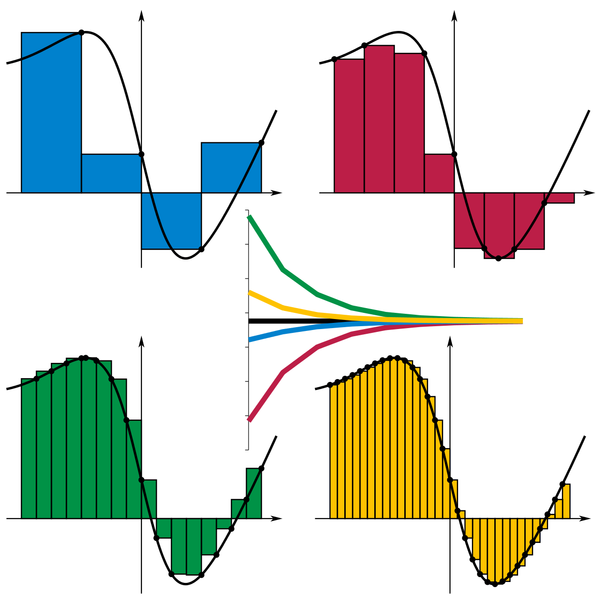
\includegraphics[scale=2]{suma_calek}}
\caption{Przykład sum Riemanna}
\end{figure}

\end{document}
